\section{Energetic particles in the heliosphere}
\label{sec:particles_heliosphere}


Our heliosphere is a vast region in space embedded in the \ac{ISM}, which encompasses all solar system planets and extends far beyond even the Kuiper belt. 
It is filled with a thin plasma consisting of various populations of particles, many of which originate from the Sun itself. These populations can be identified in \autoref{fig:heliospheric_energy_spectrum} \citep[based on measurements by][]{Mewaldt-2001}, shown as an energy spectrum that extends over more than 7 orders of 


Introduce all the particles population from lower energy to the higher energy, each population has one paragraph, according to the plot you add, and maybe one plot showed the position of multiple process, could be the plot of blue or the plot in Paddy's thesis

As shown in Fig.\ref{Fig:heliospheric_energy_spectrum}, from the lower energy end to the higher energy end, we could find several different component. Solar wind, suprathermal particle, SEP, ACR, GCR. 
The shadow region indicating the energy range between few MeV to few hundreds MeV, where SEP, ACR and GCR are co-exist. 


SEP are the particle from solar, accelerated by different mechanism.
The enery range of SEP are quite broad, especially depending the on where the measurement carried on. Recently SOLO and PSP frequently measure the hundreds keV SEP.



GCR, fully ionized particlesoriginating outside the heliosphere ,accelerated ar supernova remnants [Blasi 2013], covering the energy from typical 1MeV ([Potgieter 2023 LRSP] to ZeV, 90\% of hydrogen, the remain 10\% consist of heavier ions ( percent \%), electron, positron and antiproton (?\%)
The flux , outside the heliosphere,  is isotropic distributed in space and nearly constant in time.  It is believe the source 

ACR are the high energy interstellar particles, accelerated, ionizing,. 


Both ACR and GCR's temporal variaton is highly related with the solar activities and the so-called solar modulation, which are periodcally change in 11 and 22 year period. 

\begin{figure}
	\centering
	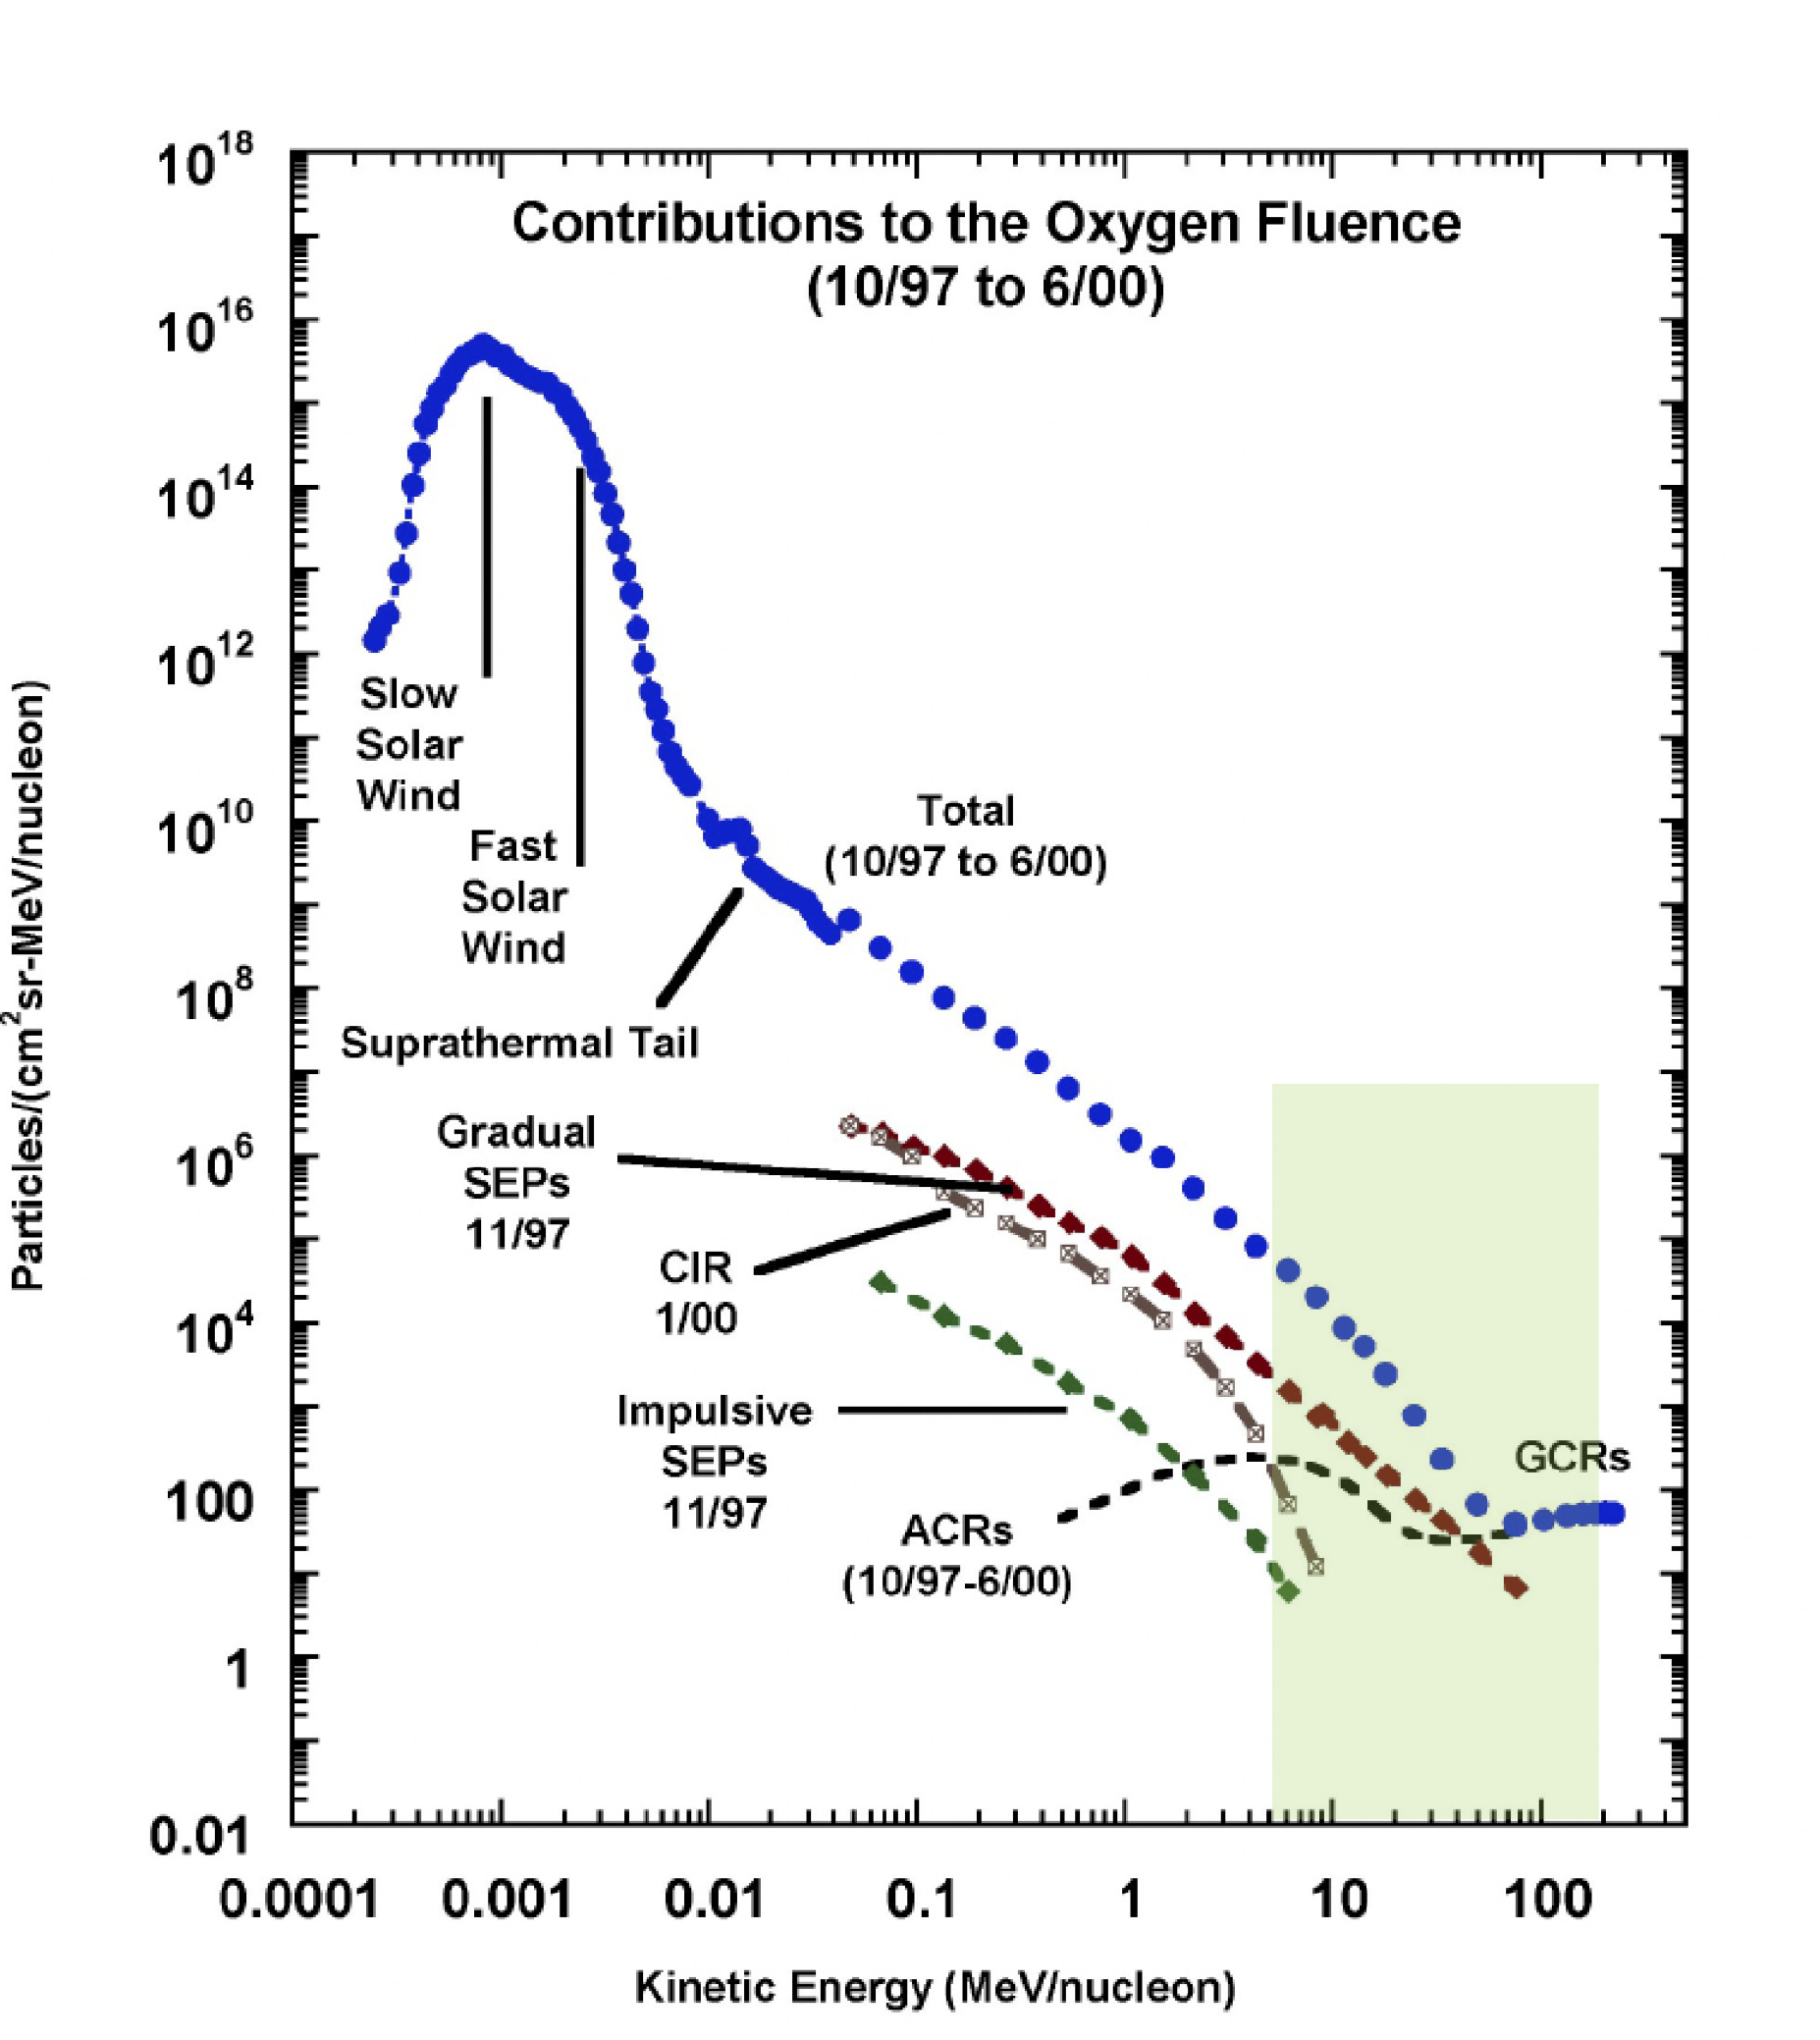
\includegraphics[width = 0.6\textwidth]{images/heliospheric_particle_spectra_color.png}
	\caption[Energy spectra of oxygen ions in the near Earth space]{The typical oxygen spectra in the interplanetary space near the Earth, indicating the contributions of different populations, especially in the energy range between few MeV\/nuc and few hundreds MeV\/nuc, where \acs{SEP}, \acs{ACR} and \acs{GCR} both exist. The spectra of other particles species for instance, helium and proton, have the similar shape but different flux level on corresponding energy region. The figure is adapted from \cite{Mewaldt-2001}}
	\label{Fig:Oxygen_spectra_heliosphere}
\end{figure}

\begin{itemize}
	\item The few tens of MeV energy range is an very important energy range for the heliosphere. In this part the SEP, ACR, lower GCR are bothe there. Therefore, more attention required here
	\item 
\end{itemize}

\section{SEP}

discovery of SEP and history of SEP
- first SEP discovery and the 
\missingfigure[options]{First SEP plot, GLE}
-  Source of SEP at 1980 - flare
 - evidence 1
 - evidence 2
 - most represented result 1
flare math
Two type of SEP and how the source of SEP evolved

Wide spread SEP
	- 
Multi-instrument observation of the SE
The problem of SEP studies



\section{Galactic cosmic rays} ( 1500 words are enough, 50 citation)

\begin{figure}
	\centering
	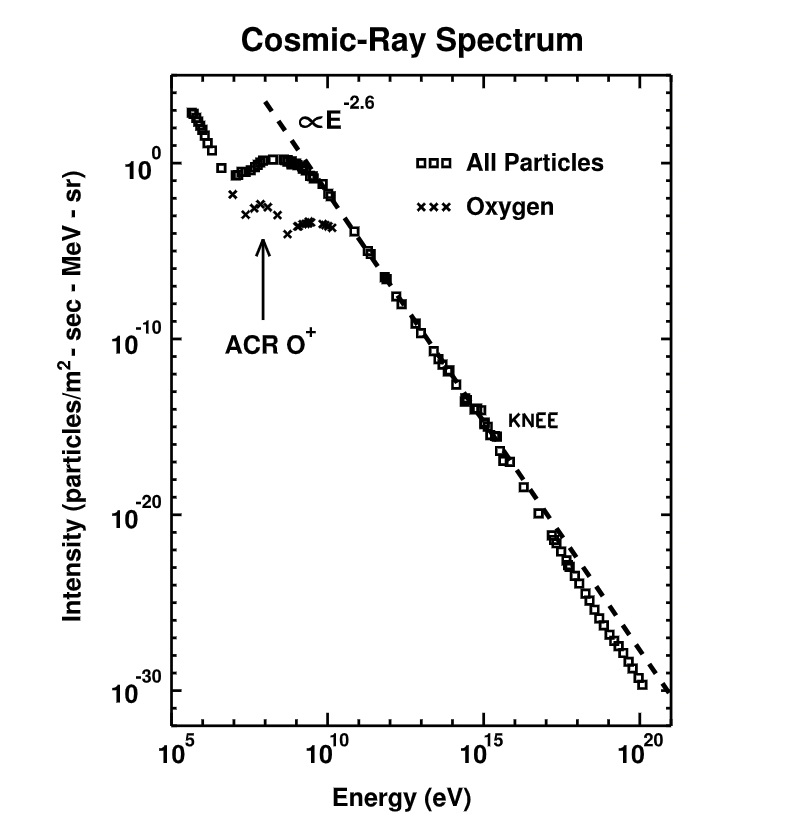
\includegraphics[width = 0.5\textwidth]{images/oxygen_cosmic-ray spectrum.png}
	
	\caption{The cosmic spectra of all particles and ACR oxygens observed at 1 AU. This figure is from Giacalone 2021, 2012, and originally from Jokipii 1990.
	The spectrum is plotted in more than 15 orders of magnitude on the energy scale and about 30 orders of magnitude on the intensity scale, extend the high energy end of Fig.\ref{Fig:Oxygen_spectra_heliosphere}.}
	\label{Fig:Oxygen_spectra_cosmic_ray}
\end{figure}
%\url{https://timeline.web.cern.ch/victor-hess-discovers-cosmic-rays-0}
The first discovery of the galactic cosmic rays was made by the Victor Hess in 1912 when he carried on a ballon experiement. The initial purpose of the experiement was to find the source of ionizing radiation in Earth's atmosphere using the electroscope. However, as the ballon climb-up in the experiment, he found that ionization rate measured in the electroscope showed less signicant decrease than anticipated. Such a discrepancy was attributed to the existence of the cosmic rays which increase the radiation in the atmoshphere.

\acs{GCR} consist of multiple energetic particle species span a wide range of energy, which are mostly dominated by the proton, about 89\%  and the remain share are 10\% helium and a small portal of heavier ions (1\%), electron, positron and antiproton. 
It is believed that \acs{GC} are mainly originated from the supernova remanent very far from the sun[citation] and obtain the energy from the shock waves which is genereated from the explosion of supernova. When the shock wave travel through the surrounding interstellar gas, the kinetic energy of shock are tranfer to the  (neutral gas?) by the (Fermi-acceleration, ciataion and the acceleration process), Utilimatly, the energetic particle with energy up to 10$^12$ eV are created.

In figure \ref{Fig:Oxyge_spectra_cosmic_ray}, the full spectrum of the all cosmic particles observed at 1 AU which includes both the \ac{ACR} and \ac{GCR} components is shown. The \acs{GCR} are indicated as empty squares. In the right half of the spectra with energy above 1 GeV, the spectrum could be simply fitted by power a law spectrum with index of about -2.6. The knee of GCR spectra are around [] energy and reflect what mechanism[citation]. The lower energy spectrum is shown as a "turn over" below 1 GeV which are more complicated and could not be fitted by a signel power law. 

% As shown in the Fig.\ref{Fig:Oxygen_spectra_heliosphere}, the dominated energy of \acs{GCR} is above 100MeV/nuc.  
% ---- To do
% [Describe the GCR spectra]
% Below that, the other component are more common than GCR and it is hard to seperated those particles.
%  ---
Because cosmic rays are fully charged, they are deflected by the magnetic field when they propagation in the interstellar space after speeding up. The directions of those particle are normalized by the strong magnetic field. Hence when they arrived at the local bubble of solar system, we obtained an nearly isotropic and constant intensity profile [citaion of the LSTM,]

To model the solar modulation on the particle transportation of GCR spectra, an input particle spectra need to be specifield, which is the so-call LSTM [ citaion of LSTM]. LSTM is the modulation boundary and will be modulatined as the change of the position, energy, and time after those particle diffusion into the heliosphere. Such a spectra have been observed by the voyeger after then cross the boundary of solar system and enter the interstellar medium.


%A paragraph of local intersteallar spectra ?

After enter the heliosphere, those high energetic particle are modulated the solar wind and its embedding magnetic field  which changes in a 11 year or 22 year period, which is so-called solar cycle.
The relavant process of the solar modulations could be described by a basic transport equation (TPE) which is first derived by Parker (1965). The same equations was also derived by Gleeson and Axford (1967) in the more rigorous ways. This equation is based on the motion of charged and particle in the high frequently changed magnetic field and averages over the pitch angle of particle moving in the magnetic field. The precondition of this equation is the reasonable assumption of the isotropically distributed GCRs. The TPE give the phase-space distribution function, $f$ as the function of positions, time and momentum magnetitude. In Potgieter (2013), the helispheric TPE, based on Parker (1965) is rewritten in the following form:

	\begin{equation}
		\underbrace{\frac{\partial f}{\partial t}}_{a} = - ( \underbrace{\boldsymbol{V}}_{b} + \underbrace{\langle v_d \rangle }_{b}) \cdot \nabla f + \underbrace{\nabla \cdot (\boldsymbol{K_s \cdot \nabla f})}_{d} + \underbrace{\frac{1}{3}(\nabla \cdot \boldsymbol{V}) \frac{\partial f}{\partial ln P}}_{d}
		\label{Eq:Transportation_equation}
	\end{equation}

where $f(r, P, t)$ is the cosmic ray distribution as the function of the time t, particle rigidity P and 3-dimension position in the space. Compared with the $\sim$ 11 years solar cycle, the periodcally solar rotation ($\sim$ 27 days) and  the time of the solar wind traveling to the edge of helipshere ($\sim$ 1 years) are short-term variation and can be neglected. Hence the steady-state solution with  $\frac{\partial f}{\partial t} = 0$ (part a of Eq.\ref{Eq:Transportation_equation}) is a reasonable assumption and also considered. Terms in the right parts include four effects that are used to describe the variation of the cosmic rays: (b) convection due to the solar wind velocity $\boldsymbol{V}$; (c) drift effects caused by the gradient and curvature of the large-scale \ac{HMF}, which is estimated by a 3D Archimedean spiral (Parker 1978), $\langle v_d \rangle$ represents the averaged drift velocity; (d) diffusion effects caused by the turbulent mangetic field, with the $\boldsymbol{K}_s$ the symmetrical diffusion tenser; (e)adiabatic energy change and deceleration due to the expansion of the solar wind. 

Since TPE is a high non-linear partial differential equation, only a simplified solution of the GCR spectra is derived which is called the Force-field Solution (FFS). The FFS was first derived by Gleeson and Axford [1967, 1968b], which simply depend on the kinetic energy T of particles and the solar modu. Later, a reasonable GCR spectra of the particle with energy above 150 MeV were given by Gleeson and Urch 1973.
With the development of computer technque and numerical studies, simulation are becoming more and more important in studying the tranporation and solar modulation of the cosmic rays. [Jokippi and Kopriva 1979, Le Roux and Potgieter 1995, Manuel et al 2011, and Potgieter 2013, Vos \& Potgieter 2015, 2016; Boschini et al. 2019;
Corti et al. 2019; Shen et al. 2019 \url{https://iopscience.iop.org/article/10.3847/2041-8213/acbea7/pdf}]. 
Several popular used model like BON14, 2020, CREME 96 and HELMOD based the solar modulation and sunspot numbers could easily reproduce the GCR intemnsity and spectra which are consistent with the measurements from \ac{ACE} in 1 AU and Voyager probes in the different regions of helisophere [Boschini et al 2019- Model]

\begin{figure}
	\centering
	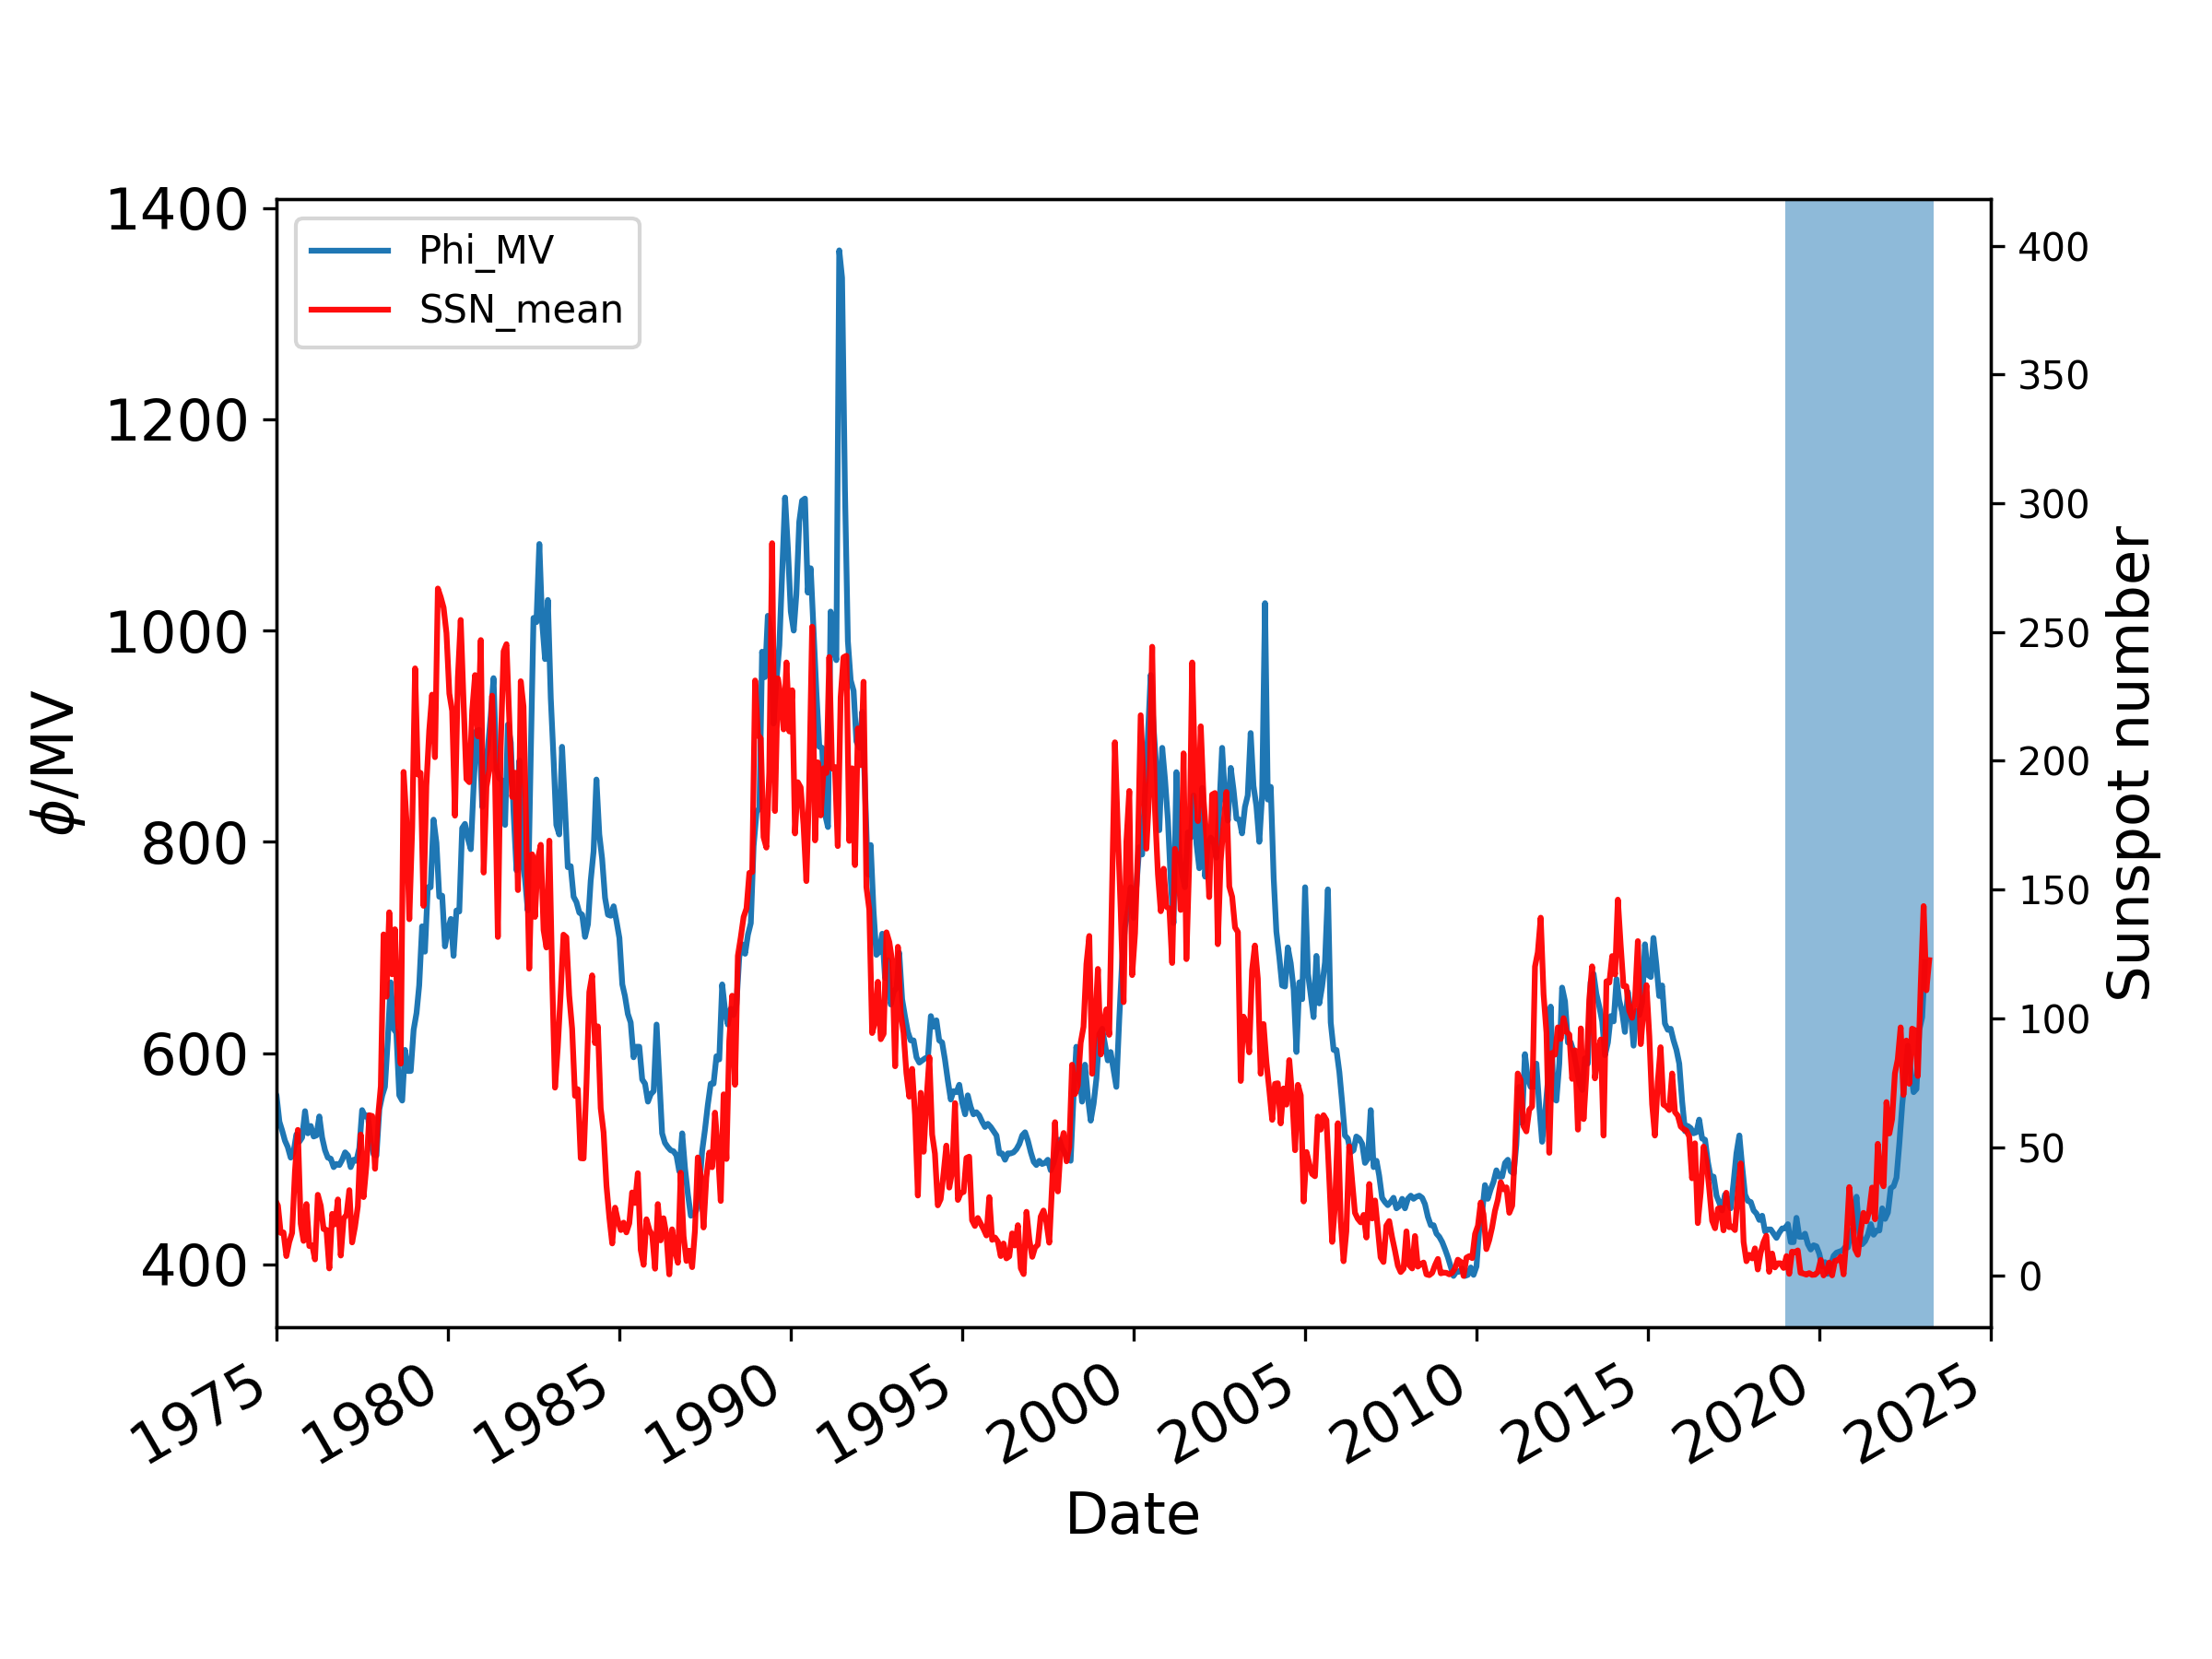
\includegraphics[width = 0.6\textwidth]{images/Solar_modulation.png}
	\caption{The solar modulation potential ($\phi$) \cite{Usoskin 2011}, data are downloaded from \url{https://cosmicrays.oulu.fi/phi/phi.html}, and the monthly averaged sunspot number from Solar Influences Data analysis Center (SIDC), Royal Observatory of Belgium, Brussels, \url{https://www.sidc.be/silso/datafiles}}
	\label{Fig:Solar_modulation}
\end{figure}


Figure \ref{Fig:Solar_modulation} show the monthly averaged sunspot number since 1975 in red and the solar modulation potential ($\phi$) \cite{Usoskin 2011}.
Sunspot number is a proxy for the solar activities. The variation of the solar modulation potential align with the variation of solar activities in the solar cycle.
The GCR flux is anti-correlated with the averaged sunspot number, that is the GCR flux peaks when the sunspot number is minimum during solar minimum and vice versa in the solar maximum.
The time between two neighbouring solar minimum is about 11 years, which is the period of the solar cycle and caused by the polarity reversal of the solar magnetic field, which is the solar cycle.

Besides the magnetic field reversal, the drift effects play an important role in the 22-year cycle of the intensity of cosmic rays. Such effects are clearly observed in the temperoal variations.
As shown in Fig.\ref{Fig:Solar_modulation}, during the A < 0 cycle, GCR had a more peaked time profile than A > 0 cycle, which have a plateau-like profile. 
This because in the A < 0 magnetic polarity cycle, the positively (negatively) charged particles drift inwards (outwards) mainly along the equatuorial plane in the heliosphere and drift outward (inwards) through the open mangentic field in the polar region, resulted the sharp change of the intensity. While in the A > 0 cycle, the drift direction of the particle is opposite to the A < 0 cycle, caused the plateau region on the solar minimum. Fig.~\ref{Fig:drift_effect} illustrate the drift effects in the opposite polarity cycles, showing the drift directions of the positively charged particles like helium, oxygen.

\begin{figure}
	\centering
	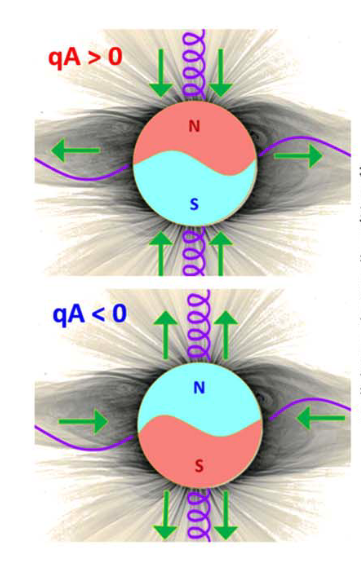
\includegraphics[width = 0.6\textwidth]{images/drift_effect.png}
	\caption{The illustration of the drift effects, adapted from the Fig. 4 of \citep{Rankim 2020?}}
	\label{Fig:drift_effect}	
\end{figure}

Furthermore, the drift effects are also reflected in the spatial gradient [Vos and Potgieter 2016] of the cosmic rays. 
\TODO{add more here}
The spatial gradient, including the latitude and radial gradients have already been observed by multiple missions for the region from 1 AU to the edge of the heliosphere in the past few solar cycles, for instance the two Voyager probes, the Ulysses spacecraft, Pioneer and also combined the measurements like PAMELA from L1 point, [citaion]
Besides, the charge sign-dependent radial gradients have been measured, finding the positive and negative latitude gradients in the outer helisphere. [citaion]


As ** indicating the solar minimum of SC 23/24 was quite unusual, with a much weaker \ac{HMF} compared with the history record and a higher then ever GCRn intensity. Further more, The recent solar minimum 
is even more unusual, the highest GCR intensity in the history and the unusual ACR intensity [that paper]. 

Therefore, the studies of both the temperal variation and spatial gradient are still not compeleted and it is still worthwhile to check the GCR data with more new data and by more detailed analysis.
	


\subsection{Anomalous Cosmic Ray}

Anomalous cosmic rays are mostly the singly charged energetic particle dominated the energy range between few meV/nuc to $\sim$ 100 MeV/nuc. \acs{ACR} were firstly discovered by the \acs{IMP} 7 and 8 in 1970s [citation]. By analyzing the lower spectra of cosmic rays, [who] et al found an "unusual" enhancement of the flux of [particle species]. As the oxygen spectra in Figure \ref{Fig:Oxygen_spectra_cosmic_ray}, the intensity of oxygen did not decrease as the energy decrease from hundred MeV/nuc to MeV/nuc, but incrase
Currently, both ACR helium, oxygen, neon, protons have been found in the outside of 1 AU region and what find in 1 AU

It is believe that ACRs are the high energy interstellare pick up ions which are accelerated in termination shock of the heliosphere. Extend this to a paragraph;
The possible acceleration mechanisam of the ACR include  (citaion)

One of the key chararcters of ACR is that those energy particles are singly charged, which could help use to seperate the ACR from the GCR and SEPs. [Find a paragraph to extend the charge state analysis]


Though the source of ACR and GCR are total different, after they entering the heliosphere, the energetic particles endourver the same transport process and interact with the solar wind and magnetic field,  which together could be described by the TPE equation.

By 1 AU, similar to GCR intensity, ACR intensities are also heaviely modulated during their transportation in the solar wind and globar \ac{HMF}. Figure \ref{Fig:ACR_solarmodulation} show the comparison between the ACR oxygen intensity and the neutron monitor count rate which is a proxy of the GCR variation in the deep space. The peaked and plateau-shaped profiles in the last two and half solar cycles are consistent in two measurements.


\begin{figure}
	\centering
	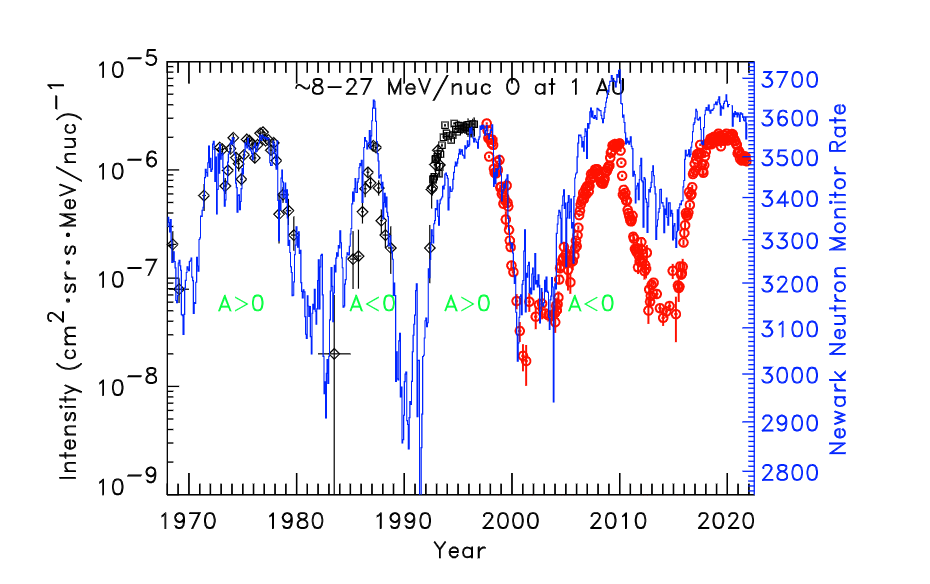
\includegraphics[width = 0.5\textwidth]{images/ACR_solarmodulation.png}
	\caption{ACR oxygen intensity with energy between 8 and 27 MeV/nuc at 1 AU measured by ACE/SIS instrument (red) and count rate of Newark Neutron monitor (blue). The plot is adapted from Figure 6 of Giacalone et al 2022}
	\label{Fig:ACR_solarmodulation}
\end{figure}

The spatial gradient consist the important information of the transportation and acceleration of the ACRs in the heliosphere and in the terminaton shock \cite{Rankin 2020}. 
The radial and latitude gradient of ACR in the region outside of 1AU

Below 1 AU, Marqunet, Helios, number 
And more recently, Rankin, PSP, find Oxygen and protons

\subsection{Radiation hazard of energetic particle and the interaction with the planet for instance Moon and Mars}

Radiation hazard of the SEP 
- Space
- on the planetary environment
Radiation from GCR and the secondary particle generated by the GCR

- GCR interaction with regolith, lunar-
	- Generation of Neutron

The exploration of space has witnessed a surge in intensity, with an increasing number of countries aspiring to venture into this domain. Noteworthy examples include NASA's initiation of the Artemis mission, which aims to return to the Moon by 2024. Similarly, China has unveiled its plans to establish a lunar base on the lunar surface by the 2030s, while the European Space Agency (ESA) has also embarked on a lunar lander mission. Most recently, a Japanese lunar lander mission was launched; however, it regrettably encountered failure.

Under these circumstances, the study of solar energetic particles (SEPs) assumes greater significance. SEPs pose a significant radiation hazard for future human exploration on the lunar surface. The most hazardous SEP events have the potential to induce radiation increases of substantial magnitude.

\subsection{Motivition}
New instrument, new data, 
Now observation point.
new solar cycle, special solar Cycle
new solar minimum, special solar minimum
